

The JuPyTer notebook is to be found at:

\url{https://github.com/ashimrijal/uu_gravity_exercises_2020}


\subsubsection{Background}

We have seen that the calculation of the gravity vector and/or the gravity potential 
for a mass distribution in 3D space is of the form 
\[
\xi(\vec{r})= {\cal G}  \int_V f(\vec{r},\vec{r}') \rho(\vec{r}') d\vec{r}'
\]
where $\xi$ is either $g_x$, $g_y$, $g_z$ or $U$ and $f$ is a function of the coordinates $\vec{r}$
and $\vec{r}'$.

Let us now assume that the body under consideration can be subdivided into $N_e$ smaller blocks/elements.
But virtue of the linearity of the integral, we have
\[
\xi(\vec{r})={\cal G} \sum_{e=1}^{N_e} \int_{V_e} f(\vec{r},\vec{r}') \rho(\vec{r}') d\vec{r}'
\]
We can further assume that inside each element the density is constant so that 
\[
\xi(\vec{r})={\cal G} \sum_{e=1}^{N_e} \rho_e \int_{V_e} f(\vec{r},\vec{r}') d\vec{r}'
\]
We will now make a strong assumption which is only valid when elements are (very) small:
we will assume that we can replace $f(\vec{r},\vec{r}')$ by $f(\vec{r},\vec{r}_e)$
where $\vec{r}_e$ is the location of the 'center' of the element. We then get:
\[
\xi(\vec{r})= {\cal G}\sum_{e=1}^{N_e} \rho_e  f(\vec{r},\vec{r}_e) \int_{V_e}d\vec{r}'
\]
And finally the integral term is simply the volume of the element $V_e$:
\[
\xi(\vec{r})= {\cal G} \sum_{e=1}^{N_e} \rho_e  f(\vec{r},\vec{r}_e) V_e
\]
In the end, assuming that the body of interest can be split into many small 
elements of constant density, the gravity fields at a location $\vec{r}=(x,y,z)$
can be computed as follows:
\[
g_x(x,y,z) = {\cal G} \sum_{e=1}^{N_e} \rho_e V_e  \frac{x-x_e}{|\vec{r}-\vec{r}_e|^3}
\]
\[
g_y(x,y,z) = {\cal G} \sum_{e=1}^{N_e} \rho_e V_e  \frac{y-y_e}{|\vec{r}-\vec{r}_e|^3}
\]
\[
g_z(x,y,z) = {\cal G} \sum_{e=1}^{N_e} \rho_e V_e  \frac{z-z_e}{|\vec{r}-\vec{r}_e|^3}
\]
\[
U(x,y,z) = -{\cal G} \sum_{e=1}^{N_e} \rho_e V_e  \frac{1}{|\vec{r}-\vec{r}_e|}
\]
where 
\[
|\vec{r}-\vec{r}_e|=\sqrt{ (x-x_e)^2+(y-y_e)^2+(z-z_e)^2   }
\]

The following exercises are designed to test this approach which lends itself to 
numerical implementation. 
The basic idea is rather simple: generate a cloud of points in a regular manner such that 
we can assign them a corresponding volume and a density when they are in the geometry of interest, 
and then use the formula above to compute the gravity vector and potential, and finally 
compare these values with the analytical solutions we derived for simple spherical bodies. 


%........................................
\subsubsection*{Exercise 1: Full sphere}

\begin{itemize}
\item In a domain of size $2R\times 2R \times 2R$ centered on the origin compute and store the coordinates 
of $N^3$ points (use $R=6371$km). Please use arrays {\tt x}, {\tt y} and {\tt z} to store the coordinates.
These arrays are $N^3$ long.\\
Help: draw on paper a $3\times3\times3$ grid. Place the axis system on the plot and explicitely write the arrays 
for all 27 points. Example:
\begin{verbatim}
x1=..... y1=..... z1=.....
x2=..... y2=..... z2=.....
...
x27=.... y27=.... z27=....
\end{verbatim}
Once you have done so, run your code for $N=3$, print the arrays and compare their content with what you 
have on paper. \\

\begin{center}
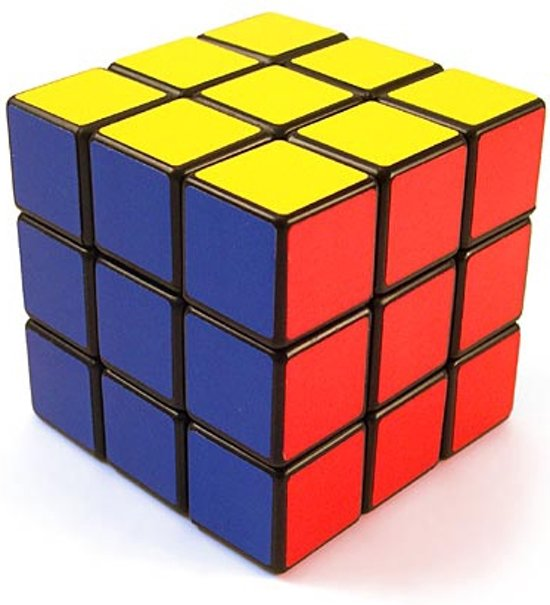
\includegraphics[width=4cm]{images/gravity/rubik}
\end{center}

Important remark: the coordinates are those of the center of the cells!




\item Compute the associated volume $dV$ of a point as a function of $R$ and N.
\item For points inside a sphere of radius $R$ assign a density $\rho_0=3000$kg/m$^3$ and zero otherwise, store these values in the {\tt rho} array.
\item Compute the total mass of the system 
\item Compute the moment of inertia of the system and compare the obtained value with its analytical value 
(obtained with Eq. \ref{mominert_uniform_sphere}). In order to compute this quantity we will make use of
the formula for a spherically symmetric body: 
\[
I = \int_V \rho d^2 dV \simeq \sum_i \rho_i d_i^2 dV_i
\]
where $d_i$ is the distance of point $i$ to the axis.

\item Compute the gravity potential and vector components at $z=H=10^m$ meters above the north pole 
with $m=0,1,2,3,..8$. Compute first the position of these points and store them 
in arrays {\tt xm}, {\tt ym} {\tt zm} before using these for gravity calculations. 
\item Plot the computed quantities as a function of $H$ and plot on the same graphic the analytical values. 
\item Repeat the exercise with different values of $N\in(10,20,30,40,50)$ .
For the mass and moment of inertia, plot the relative error as a function of $h$.
Discuss.
\item Fix $m=4$. Progressively increase $N$ and record the absolute error on the gravity vector norm 
as a function of $dV^{1/3}$. Plot this in log-log scale. Discuss.
\item Use the {\tt prem\_density} function to assign the density to the points. Compute the mass of the planet with this new density distribution and compare it with the mass of the Earth. Compute the gravity at the surface.
\end{itemize}

%..........................................
\subsubsection*{Exercise 2: Hollow sphere}

This is based on the previous exercise. 
\begin{itemize}
\item For points with radius $r$ such that $R/2 \le r \le R$ assign a density $\rho_0=3000$kg/m$^3$ 
and zero otherwise.
\item Compute the gravity potential and vector components on the $x$ axis between $r=0$ and $r=3R$ 
with steps of $R/100$.
\item Plot the results and the analytical solution on the same plot as a function of $r$.
\item Repeat the exercise with different values of $N$. Discuss.
\end{itemize}

%....................................................
\subsubsection*{Exercise 3: Full sphere - revisited}

We are now going to re-do the first exercise but this time we do not want any point outside of the sphere. 
We shall therefore use the spherical coordinates (see Section~\ref{ss:sphercoord}).
We will use three for loops, one over $r\in[0,R]$ values, 
one over $\theta\in[0,\pi]$ values and one over $\phi\in]-\pi,\pi]$ values. The number 
of points in each direction in this space is still $N$ so that the total number of points is
still $N^3$.

\begin{itemize}
\item Compute and store the coordinates of the points in the $r,\theta,\phi$ space. Store 
these in arrays {\tt r}, {\tt theta}, {\tt phi}.
\item Use these coordinates to compute and store the Cartesian coordinates of these points. 
\item Plot this cloud of points in 3D. Discuss.
\item Repeat the calculations of the first exercise.
\item The cost of the calculation is the same as in exercise 1, but what about accuracy?
\end{itemize}


%what is the resolution one would need to represent the ellipsity of the Earth ?
% compute then moments of inertia
% look at McCullagh formula

%............................................
%\subsubsection{Full sphere - revisited again}
%\url{https://stackoverflow.com/questions/9600801/evenly-distributing-n-points-on-a-sphere/44164075#44164075}
%\begin{lstlisting}
%from numpy import pi, cos, sin, arccos, arange
%import mpl_toolkits.mplot3d
%import matplotlib.pyplot as pp
%num_pts = 1000
%indices = arange(0, num_pts, dtype=float) + 0.5
%phi = arccos(1 - 2*indices/num_pts)
%theta = pi * (1 + 5**0.5) * indices
%x, y, z = cos(theta) * sin(phi), sin(theta) * sin(phi), cos(phi);
%pp.figure().add_subplot(111, projection='3d').scatter(x, y, z);
%pp.show()
%\end{lstlisting}
%\subsubsection{Crust 1.0? s40rts ? }
%measure at random lat lon instead of north pole
